%%%%%%%%%%%%%%%%%%%%%%%%%%%%%%%%%%%%%%%%%%%%%%%%%%%%%%%%%%%%%%%%%%%%%%%%%%%%%%%%
%%%%%%%%%%%%%%%%%%%%%%%%%%%%%%%%%%%%%%%%%%%%%%%%%%%%%%%%%%%%%%%%%%%%%%%%%%%%%%%%
%%% Template for AIMS Rwanda Assignments         %%%              %%%
%%% Author:   AIMS Rwanda tutors                             %%%   ###        %%%
%%% Email: tutors2017-18@aims.ac.rw                               %%%   ###        %%%
%%% Copyright: This template was designed to be used for    %%% #######      %%%
%%% the assignments at AIMS Rwanda during the academic year %%%   ###        %%%
%%% 2017-2018.                                              %%%   #########  %%%
%%% You are free to alter any part of this document for     %%%   ###   ###  %%%
%%% yourself and for distribution.                          %%%   ###   ###  %%%
%%%                                                         %%%              %%%
%%%%%%%%%%%%%%%%%%%%%%%%%%%%%%%%%%%%%%%%%%%%%%%%%%%%%%%%%%%%%%%%%%%%%%%%%%%%%%%%
%%%%%%%%%%%%%%%%%%%%%%%%%%%%%%%%%%%%%%%%%%%%%%%%%%%%%%%%%%%%%%%%%%%%%%%%%%%%%%%%


%%%%%% Ensure that you do not write the questions before each of the solutions because it is not necessary. %%%%%% 

\documentclass[12pt,a4paper]{article}

%%%%%%%%%%%%%%%%%%%%%%%%% packages %%%%%%%%%%%%%%%%%%%%%%%%
\usepackage{amsmath}
\usepackage{amssymb}
\usepackage{amsthm}
\usepackage{amsfonts}
\usepackage{graphicx}
\usepackage[all]{xy}
\usepackage{actuarialsymbol}
\usepackage{actuarialangle}
\usepackage{tikz}
\usepackage{verbatim}
\usepackage[left=2cm,right=2cm,top=3cm,bottom=2.5cm]{geometry}
\usepackage{hyperref}
\usepackage{caption}
\usepackage{subcaption}
\usepackage{psfrag}

%%%%%%%%%%%%%%%%%%%%% students data %%%%%%%%%%%%%%%%%%%%%%%%
\newcommand{\student}{Akor Stanley}
\newcommand{\course}{NMC }
\newcommand{\assignment}{2}

%%%%%%%%%%%%%%%%%%% using theorem style %%%%%%%%%%%%%%%%%%%%
\newtheorem{thm}{Theorem}
\newtheorem{lem}[thm]{Lemma}
\newtheorem{defn}[thm]{Definition}
\newtheorem{exa}[thm]{Example}
\newtheorem{rem}[thm]{Remark}
\newtheorem{coro}[thm]{Corollary}
\newtheorem{quest}{Question}[section]

%%%%%%%%%%%%%%  Shortcut for usual set of numbers  %%%%%%%%%%%

\newcommand{\N}{\mathbb{N}}
\newcommand{\Z}{\mathbb{Z}}
\newcommand{\Q}{\mathbb{Q}}
\newcommand{\R}{\mathbb{R}}
\newcommand{\C}{\mathbb{C}}
%%%%%%%%%%%%%%%%%%%%%%%%%%%%%%%%%%%%%%%%%%%%%%%%%%%%%%%555
\begin{document}
%%%%%%%%%%%%%%%%%%%%%%% title page %%%%%%%%%%%%%%%%%%%%%%%%%%
\thispagestyle{empty}
\begin{center}
\textbf{AFRICAN INSTITUTE FOR MATHEMATICAL SCIENCES \\[0.5cm]
(AIMS RWANDA, KIGALI)}
\vspace{1.0cm}
\end{center}
%%%%%%%%%%%%%%%%%%%%% assignment information %%%%%%%%%%%%%%%%
\noindent
\rule{17cm}{0.2cm}\\[0.3cm]
Name: \student \hfill Assignment Number: \assignment\\[0.1cm]
Course: \course \hfill Date: \today\\
\rule{17cm}{0.05cm}
\vspace{1.0cm}
\section*{Question 1}
Given
\begin{align*}
D_{2}u(\bar{x})=\frac{\alpha u(\bar{x})+\beta u(\bar{x}-h)+\gamma u(\bar{x}-2h)}{h}
\end{align*}
We are interested in finding the values of the constants; $\alpha,\beta,\gamma$.
\begin{align*}
\beta u(\bar{x}-h)&=\beta\left[u(\bar{x})-hu^{\prime}(\bar{x})+\frac{h^{2}}{2}u^{\prime \prime}(\bar{x})-\frac{h^{3}}{6}u^{\prime \prime \prime}(\bar{x})+\frac{h^{4}}{24}u^{\prime \prime \prime \prime}(\bar{x})-\frac{h^{5}}{120}u^{\prime \prime \prime \prime \prime}(\bar{x}) + 0(h^{6})\right]\\
\gamma u(\bar{x}-2h)&=\gamma\left[u(\bar{x})-2hu^{\prime}(\bar{x})+2h^{2}u^{\prime \prime}(\bar{x})-\frac{4h^{3}}{3}u^{\prime \prime \prime}(\bar{x})+ \frac{2h^{4}}{3}u^{\prime \prime \prime \prime}(\bar{x}) -\frac{4h^{5}}{15}u^{\prime \prime \prime \prime \prime}(\bar{x}) + 0(h^{6})\right]\\
\alpha u(\bar{x})&=\alpha u(\bar{x})
\end{align*}
Thus we shall have;
\begin{align*}
u(\bar{x}-h)+ u(\bar{x}-2h)+\alpha u(\bar{x}&)=(\alpha+\beta+\gamma)u(\bar{x})+h(-\beta -2\gamma)u^{\prime}(\bar{x})+h^{3}(-\frac{1}{6}\beta-\frac{4}{3}\gamma)u^{\prime \prime \prime}(\bar{x})\\
D_{2}u&=(\bar{x})\frac{1}{h}\left((\alpha+\beta+\gamma)u(\bar{x})+h(-\beta -2\gamma)u^{\prime}(\bar{x})+h^{2}\left(\frac{\beta +4\gamma }{2}\right)\right)
\end{align*}
Since we want to approximate the first derivative, we can obtain a system of equations given by
\begin{align*}
\begin{cases}
\alpha+\beta+\gamma&=0\\
-\beta -2\gamma&=1\\
\beta +4\gamma&=0
\end{cases}
\end{align*}
By solving the system of equations simultaneously, we obtain
$$\alpha=\frac{3}{2}, \quad \beta=-2, \quad \gamma=\frac{1}{2}$$
\section*{Question 2}
\begin{itemize}
	\item [(1)]
	We want to show that
	\begin{align*}
	Du(x_{i+\frac{1}{2}})=\frac{u(x_{i+1})-u(x_{i})}{h}
	\end{align*}
	We know that the central scheme is obtained by averaging the forward and the backward schemes, that is;
	\begin{align*}
	Du(x_{i+\frac{1}{2}})=\frac{1}{2}\left(D_{-}u(x_{i+\frac{1}{2}})+D_{+}u(x_{i+\frac{1}{2}})\right)
	\end{align*}
	But
	\begin{align*}
	D_{-}u(x_{i+\frac{1}{2}})&=\frac{u(x_{i+\frac{h}{2}})-u(x_{i})}{\frac{h}{2}}\approx u^{\prime}(x_{i+\frac{1}{2}})\\
		D_{+}u(x_{i+\frac{1}{2}})&=\frac{u(x_{i+\frac{h}{2}+\frac{h}{2}})-u(x_{i+\frac{h}{2}})}{\frac{h}{2}}\approx u^{\prime}(x_{i+\frac{1}{2}})
	\end{align*}
	Since $x_{i+\frac{1}{2}}=x_{i+\frac{h}{2}}$, we shall then have;
	\begin{align*}
		Du(x_{i+\frac{1}{2}})&=\frac{1}{2}\left(\frac{u(x_{i+\frac{1}{2}})-u(x_{i})}{\frac{h}{2}}+\frac{u(x_{i+1})-u(x_{i+\frac{1}{2}})}{\frac{h}{2}}\right)\\
	Du(x_{i+\frac{1}{2}})&=\frac{u(x_{i+1})-u(x_{i})}{h}\approx u^{\prime}(x_{i+\frac{1}{2}})
	\end{align*}
	Hence shown!
	\item[(2)]
	We want to find the approximate of $v(x_{i+\frac{1}{2}}).$
	Given
	\begin{align*}
	v(x)=K(x)u^{\prime}(x)
	\end{align*}
	Therefore;
	\begin{align}
	v\left(x_{i+\frac{1}{2}}\right)&=K\left(x_{i+\frac{1}{2}}\right)u^{\prime}\left(x_{i+\frac{1}{2}}\right) \label{1}
	\end{align}
	But
	\begin{align*}
	u^{\prime}\left(x_{i+\frac{1}{2}}\right)=\frac{u\left(x_{i+1}\right)-u\left(x_{i}\right)}{h}
	\end{align*}
	Thus equation\ref{1}, becomes;
	\begin{align}
		v\left(x_{i+\frac{1}{2}}\right)&=K\left(x_{i+\frac{1}{2}}\right)\frac{u\left(x_{i+1}\right)-u\left(x_{i}\right)}{h} \label{3}
	\end{align}
	\item[(3)]
	We want to show $Dv(x_{i})$ is a central approximation of $v^{\prime}(x_{i})$, where;
	\begin{align*}
	Dv(x_{i})=\frac{v\left(x_{i+\frac{1}{2}}\right)-v\left(x_{i-\frac{1}{2}}\right)}{h}
	\end{align*}
	We know that a central approximation is defined by;
	\begin{align*}
	Du(x_{i})=\frac{1}{2}\left(D_{-}u(x_{i})+D_{+}u(x_{i})\right)
	\end{align*}
	Thus
	\begin{align*}
	D_{+}v(x_{i})&=\frac{v\left(x_{i+\frac{h}{2}}\right)-v\left(x_{i}\right)}{\frac{h}{2}} \approx v^{\prime}(x_{i})\\
	D_{-}v(x_{i})&=\frac{v\left(x_{i}\right)-v\left(x_{i-\frac{h}{2}}\right)}{\frac{h}{2}} \approx v^{\prime}(x_{i})\\
	Dv(x_{i})&=\frac{1}{2}\left(\frac{v\left(x_{i+\frac{h}{2}}\right)-v\left(x_{i}\right)}{\frac{h}{2}}+\frac{v\left(x_{i}\right)-v\left(x_{i-\frac{h}{2}}\right)}{\frac{h}{2}}\right)\\
	&=\frac{1}{2}\left(\frac{v\left(x_{i+\frac{1}{2}}\right)-v\left(x_{i}\right)}{\frac{h}{2}}+\frac{v\left(x_{i}\right)-v\left(x_{i-\frac{1}{2}}\right)}{\frac{h}{2}}\right)\\
	Dv(x_{i})&=\frac{v\left(x_{i+\frac{1}{2}}\right)-v\left(x_{i-\frac{1}{2}}\right)}{h} \approx v^{\prime}(x_{i})
	\end{align*}
	Hence shown!
	\item[(4)]
	We want to show that
	\begin{align*}
	D^{2}u(x_{i})&=\frac{1}{h^{2}}\left(\left(K\left(x_{i-\frac{1}{2}}\right)u\left(x_{i}-1\right)-K\left(x_{i-\frac{1}{2}}\right)+K\left(x_{i+\frac{1}{2}}\right)\right)u(x_{i})+K\left(x_{i+\frac{1}{2}}\right)u(x_{i+1})\right)
	\end{align*}
	is the approximate of $\left(kv^{\prime}\right)^{\prime}(x_{i})$\\
	\newline
	we know that;
	\begin{align*}
	v(x_{i})&=k(x_{i})u^{\prime}(x_{i})\\
	v(x_{i})^{\prime}&=(k(x)u^{\prime})^{\prime}(x_{i})
	\end{align*}
	But
	\begin{align*}
	v(x_{i})^{\prime} &\approx Dv(x_{i})=\frac{v\left(x_{i+\frac{1}{2}}\right)-v\left(x_{i-\frac{1}{2}}\right)}{h}
	\end{align*}
	From equation\ref{3}, we already obtained $v\left(x_{i+\frac{1}{2}}\right)$, from which we can also infer for $v\left(x_{i-\frac{1}{2}}\right)$
	\begin{align*}
	v(x_{i})^{\prime}&=\frac{1}{h}\left(K\left(x_{i+\frac{1}{2}}\right)\frac{u\left(x_{i+1}\right)-u\left(x_{i}\right)}{h}-K\left(x_{i-\frac{1}{2}}\right)\frac{u\left(x_{i}\right)-u\left(x_{i-1}\right)}{h}\right)\\
	&\frac{1}{h^{2}}\left[K\left(x_{i+\frac{1}{2}}\right)u\left(x_{i+1}\right)-\left(K\left(x_{i+\frac{1}{2}}\right)+K\left(x_{i-\frac{1}{2}}\right)\right)u\left(x_{i}\right)+K\left(x_{i-\frac{1}{2}}\right)u\left(x_{i-1}\right)\right]
	\end{align*}
	Hence shown!
	
	\item[(5)] 
	\begin{align*}
	PH
	\begin{cases}
	\frac{1}{h^{2}}\left(-K_{i-\frac{1}{2}}U_{i-1}+\left(K_{i-\frac{1}{2}}+K_{i+\frac{1}{2}}\right)U_{i}-K_{i+\frac{1}{2}}U_{i+1}\right)&=f(x_{i}) \quad \quad \forall 1 \leq i\leq N-1\\
	U_{0}=\alpha; \quad U_{N}=\beta
	\end{cases}
	\end{align*}
	We want to express PH in the matrix form $AU=F$, where $A, U$ and $F$ have to be determined.
	\begin{align*}
	-K_{i-\frac{1}{2}}U_{i-1}+\left(K_{i-\frac{1}{2}}+K_{i+\frac{1}{2}}\right)U_{i}-K_{i+\frac{1}{2}}U_{i+1}&=h^{2}f(x_{i})\\
	for \quad i=1: -K_{\frac{1}{2}}U_{0} +\left(K_{\frac{1}{2}}+K_{\frac{3}{2}}\right)U_{1}-K_{\frac{3}{2}}U_{2} &=h^{2}f(x_{1})\\
	for \quad i=2: -K_{\frac{3}{2}}U_{1}+\left(K_{\frac{3}{2}}+K_{\frac{5}{2}}\right)U_{2}-K_{\frac{5}{2}}U_{3}&=h^{2}f(x_{2})\\
	for \quad i =3: -K_{\frac{5}{2}}U_{2}+\left(K_{\frac{5}{2}}+K_{\frac{7}{2}}\right)U_{3}-K_{\frac{7}{2}}U_{4}&=h^{2}f(x_{3})\\
	\vdots \qquad \vdots \qquad 	\vdots \qquad \qquad \vdots \qquad \vdots \qquad \vdots \qquad \vdots \qquad \vdots\\
	%for \quad i=N-2: -K_{N-\frac{5}{2}}U_{N-3}+\left(K_{N-\frac{5}{2}}+K_{N-\frac{3}{2}}\right)U_{N-2}-K_{N-\frac{3}{2}}U_{N-1}&=f(x_{N-2})\\
	for \quad i=N-1:-K_{N-\frac{3}{2}}U_{N-2}+\left(K_{N-\frac{3}{2}}+K_{N-\frac{1}{2}}\right)U_{N-1}-K_{N-\frac{1}{2}}U_{N}&=f(x_{N-1})
	\end{align*}
	Representing the above in matrix form, we obtain;
	$$AU=F$$
	\begin{align*}
	&\begin{bmatrix}
	K_{\frac{1}{2}}+K_{\frac{3}{2}}& -K_{\frac{3}{2}}  & 0&0& \cdots&0 \\
	-K_{\frac{3}{2}}& K_{\frac{3}{2}}+K_{\frac{5}{2}}&-K_{\frac{5}{2}}&0&\cdots&0
	\\
	0&-K_{\frac{5}{2}}&K_{\frac{5}{2}}+K_{\frac{7}{2}}&-K_{\frac{7}{2}}&\cdots&0&\\
	\vdots& \vdots&\vdots\\
	0 &\cdots&0&\cdots&-K_{N-\frac{3}{2}}&K_{N-\frac{3}{2}}+K_{N-\frac{1}{2}}
	\end{bmatrix}\begin{bmatrix}
	U_{1}\\
	U_{2}\\
	U_{3}\\
	\vdots\\
	U_{N-1}
	\end{bmatrix}\\&=\begin{bmatrix}
	\alpha K_{\frac{1}{2}}+h^{2}f(x_{1})\\
	h^{2}f(x_{2})\\
	h^{2}f(x_{3})\\
	\vdots\\
	\beta K_{N-\frac{1}{2}}+h^{2}f(x_{N-1})
	\end{bmatrix}
	\end{align*}
	\item[(2)] For a matrix to be symmetric,then it must be equal to its transpose. The obtained matrix $A$ is equal to its transpose.
	$$A=A^{T}$$
	%\newline
	%Using the Sylvester's criterion, we shall evaluate the determinant of matrix A, and thus show that matrix $A$ is positive definite. The determinant of the first element is given by
	%\begin{align*}
	%det\left(K_{\frac{1}{2}}+K_{\frac{3}{2}}\right)
	%&=K_{\frac{1}{2}}+K_{\frac{3}{2}}\\
	%&0\leq 
	%\end{align*}
	%Next, we consider the $2\times2$ in matrix $A$
	%\begin{align*}
	%det\begin{pmatrix}
	%K_{\frac{1}{2}}+K_{\frac{3}{2}}&-K_{\frac{3}{2}}\\
	%-K_{\frac{3}{2}}&K_{\frac{3}{2}}+K_{\frac{5}{2}}
	%\end{pmatrix}&=\left(	K_{\frac{1}{2}}+K_{\frac{3}{2}}\right)\left(K_{\frac{3}{2}}+K_{\frac{5}{2}}\right)-\left(K_{\frac{3}{2}}\right)^{2}\\
	%&=K_{\frac{1}{2}}K_{\frac{3}{2}}+K_{\frac{3}{2}}K_{\frac{5}{2}}+K_{\frac{1}{2}}K_{\frac{5}{2}}
	%\end{align*}
	%det
	%\begin{pmatrix}
	%K_{\frac{1}{2}}+K_{\frac{3}{2}}&-K_{\frac{3}{2}}&0\\
	%-K_{\frac{3}{2}}&K_{\frac{3}{2}}+K_{\frac{5}{2}}&-K_{\frac{5}{2}}\\
	%0&-K_{\frac{5}{2}}&K_{\frac{5}{2}}+K_{\frac{7}{2}}
	%\end{pmatrix}
	%\end{align*}
	%This then yields
	%\begin{align*}
	%&\left(K_{\frac{1}{2}}+K_{\frac{3}{2}}\right)\left[\left(K_{\frac{3}{2}}+K_{\frac{5}{2}}\right)\left(K_{\frac{5}{2}}+K_{\frac{7}{2}}\right)-\left(K_{\frac{5}{2}}\right)^{2}\right]+K_{\frac{3}{2}}\left[-K_{\frac{3}{2}}\left(K_{\frac{5}{2}}+K_{\frac{7}{2}}\right)\right]\\
	%&K_{\frac{1}{2}}K_{\frac{1}{2}}\left(K_{\frac{5}{2}}+K_{\frac{7}{2}}\right)+K_{\frac{1}{2}}K_{\frac{5}{2}}K_{\frac{7}{2}}+K_{\frac{3}{2}}K_{\frac{5}{2}}K_{\frac{7}{2}}\\
	%&K_{\frac{1}{2}}K_{\frac{1}{2}}\left(K_{\frac{5}{2}}+K_{\frac{7}{2}}\right)+K_{\frac{1}{2}}\left(K_{\frac{5}{2}}+K_{\frac{3}{2}}\right)
	%\end{align*}
	%Since $K=x^{2}$, we can conclude that all the determinants evaluated will be greater than or equal to zero, hence Sylvester's Criterion is satisfied and our matrix $A$ has been proven to be positive definite.\\
	\begin{align*}
	A^{T}=\begin{bmatrix}
	K_{\frac{1}{2}}+K_{\frac{3}{2}}& -K_{\frac{3}{2}}  & 0&0& \cdots&0 \\
	-K_{\frac{3}{2}}& K_{\frac{3}{2}}+K_{\frac{5}{2}}&-K_{\frac{5}{2}}&0&\cdots&0
	\\
	0&-K_{\frac{5}{2}}&K_{\frac{5}{2}}+K_{\frac{7}{2}}&-K_{\frac{7}{2}}&\cdots&0&\\
	\vdots& \vdots&\vdots\\
	0 &\cdots&0&\cdots&-K_{N-\frac{3}{2}}&K_{N-\frac{3}{2}}+K_{N-\frac{1}{2}}
	\end{bmatrix}
	\end{align*}
	Since $A=A^{T}$, thus matrix A is symmetric.\\
	\newline
	To prove that matrix $A$ is positive define, we perform the operation $(Av,v)$ and check if it is greater than zero for all $v \in \R ^{N-1}$ and $(Av,v)=0$ if and only if $v=0$
	
	\begin{align*}
	Av=\begin{bmatrix}
	K_{\frac{1}{2}}+K_{\frac{3}{2}}& -K_{\frac{3}{2}}  & 0&0& \cdots&0 \\
	-K_{\frac{3}{2}}& K_{\frac{3}{2}}+K_{\frac{5}{2}}&-K_{\frac{5}{2}}&0&\cdots&0
	\\
	0&-K_{\frac{5}{2}}&K_{\frac{5}{2}}+K_{\frac{7}{2}}&-K_{\frac{7}{2}}&\cdots&0&\\
	\vdots& \vdots&\vdots\\
	0 &\cdots&0&\cdots&-K_{N-\frac{3}{2}}&K_{N-\frac{3}{2}}+K_{N-\frac{1}{2}}
	\end{bmatrix}\begin{bmatrix}
	v_{1}\\
	v_{2}\\
	v_{3}\\
	\vdots\\
	v_{N-1}
	\end{bmatrix}\\
	\end{align*}
	\begin{align*}
	Av&=\begin{bmatrix}
	\left(K_{\frac{1}{2}}+K_{\frac{3}{2}}\right)v_{1}  -K_{\frac{3}{2}}v_{2}\\
	-K_{\frac{3}{2}}v_{1}+ \left(K_{\frac{3}{2}}+K_{\frac{5}{2}}\right)v_{2}-K_{\frac{5}{2}}v_{3}\\
	-K_{\frac{5}{2}}v_{2}+\left(K_{\frac{5}{2}}+K_{\frac{7}{2}}\right)v_{3}-K_{\frac{7}{2}}v_{4}\\
	\vdots\\
	-K_{N-\frac{3}{2}}v_{N-2}+\left(K_{N-\frac{3}{2}}+K_{N-\frac{1}{2}}\right)v_{N-1}
	\end{bmatrix}
	\end{align*}
	Thus the sccalar product $(Av,v)$ is given by;
	\begin{align*}
	\begin{bmatrix}
	(K_{\frac{1}{2}}+K_{\frac{3}{2}})v_{1}  -K_{\frac{3}{2}}v_{2}\\
	-K_{\frac{3}{2}}v_{1}+ (K_{\frac{3}{2}}+K_{\frac{5}{2}})v_{2}-K_{\frac{5}{2}}v_{3}\\
	-K_{\frac{5}{2}}v_{2}+(K_{\frac{5}{2}}+K_{\frac{7}{2}})v_{3}-K_{\frac{7}{2}}v_{4}\\
	\vdots\\
	-K_{N-\frac{3}{2}}v_{N-2}+(K_{N-\frac{3}{2}}+K_{N-\frac{1}{2}})v_{N-1}
	\end{bmatrix}\begin{bmatrix}
	v_{1}\\
	v_{2}\\
	v_{3}\\
	\vdots\\
	v_{N-1}
	\end{bmatrix}
	\end{align*}
	Which then yields;
	\begin{align*}
	(Av,v)&=(K_{\frac{1}{2}}+K_{\frac{3}{2}})v_{1}^{2}-K_{\frac{3}{2}}v_{1}v_{2}-K_{\frac{3}{2}}v_{1}v_{2}+(K_{\frac{3}{2}}+K_{\frac{5}{2}})v_{2}^{2}-K_{\frac{5}{2}}v_{3}v_{2}-K_{\frac{5}{2}}v_{2}v_{3}+(K_{\frac{5}{2}}+K_{\frac{7}{2}})v_{3}^{2}\\
	&-K_{\frac{7}{2}}v_{4}v_{3}+\cdots+-K_{N-\frac{3}{2}}v_{N-2}v_{N-1}+(K_{N-\frac{3}{2}}+K_{N-\frac{1}{2}})v_{N-1}^{2}\\
	&=K_{\frac{1}{2}}v_{1}^{2}+K_{\frac{3}{2}}(v_{1}-v_{2})^{2}+K_{\frac{5}{2}}(v_{1}-v_{2})^{2}+K_{\frac{7}{2}}(v_{3}-v_{2})^{2}+\cdots+K_{N-\frac{3}{2}}(v_{N-2}-v_{N-1})^{2}
	\end{align*}
	For  $i,j \in \R$, Since $(v_{i}-v_{j})^{2}$ and $v_{i}^{2}$ or $v_{j}^{2}$ is always greater than or equal to zero for $i\neq j$, and given the fact that $K=x^{2}\geq0$, we can thus conclude that $(Av,v)\geq0$ and so $A$ is positive definite. 
	\newpage
	\textbf{APPLICATION}
	\begin{itemize}
		\item [(1)] Given $a=0, \quad b=1$, $K(x)=x^{2}$ and $u(x)=x(1+x)$
		\begin{align*}
		u(x)&=x(1+x)   \quad \quad x\in(0,1)\\
		u(0)&=u_{0}=0\\
		u(1)&=u_{1}=2
		\end{align*}
		Therefore $\alpha=0,\quad \beta=2.$
		\begin{align*}
		u^{\prime}&=1+2x\\
		-(ku)^{\prime}(x)&=f(x)\\
		\implies f(x)&= -(x^{2}(1+2x))^{\prime} \\
		&=-2x-6x^{2}
		\end{align*}
		\item[(3)]The figure below shows the plot of the exact and approximate solution of $(PH)$
		\begin{figure}[h!]
			\centering
			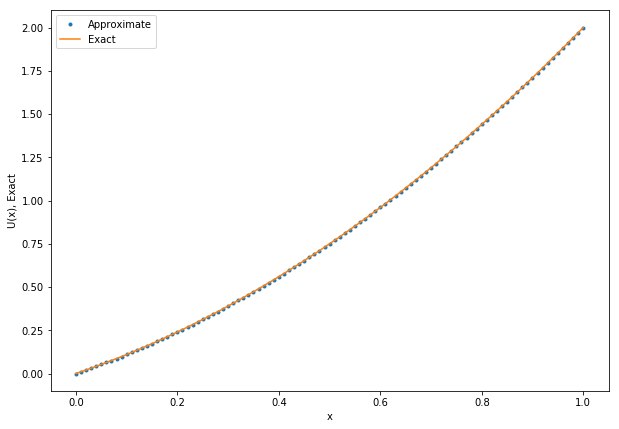
\includegraphics[scale=0.5]{1.png}
			\caption{Approximate Vs Exact Solution}
		\end{figure}
	\end{itemize}
\end{itemize}
\end{document}